% \newcommand{\xqq}{x862}

\todo[inline]{source -> ASM -> binaire // asm -> (désas) -> (décomp)}
Nous nous intéressons en premier lieu aux programmes malveillants fonctionnant sur des ordinateurs personnels.
Les programmes s'exécutant sur ces machines sont compilés afin d'être exécutés nativement dans le langage assembleur spécifique au processeur de la machine.

\section{Compilation et fichiers exécutables}
Un exécutable est en général d'abord écrit dans un langage de haut niveau. Chacun de ses modules est ensuite compilé en un fichier objet (binaire) encodant le langage assembleur spécifique à la machine. La dernière étape est l'édition de liens qui consiste à regrouper tous les fichiers objets en un exécutable unique.

Prenons l'exemple d'un simple \helloworld\ en C (Figure \ref{fig:helloword_c}). Il est uniquement composé d'un appel à la fonction \texttt{printf} permettant l'affichage, à l'exécution, de la chaîne de caractère ``Hello, world.''.
Une implémentation possible en assembleur \nasm\ \xq\ pouvant tourner sous une distribution GNU/Linux est donnée en figure \ref{fig:helloword_asm}. Il est alors composé de deux appels système vers le noyau Linux : une première (sys$\_$write) permettant l'affichage de la chaîne et une seconde (sys$\_$exit) permettant de fermer le processus.
On peut déjà remarque que le programme est séparé en une section de données (.data) contenant la chaîne de caractère à afficher et une section de code (.text) contenant le code assembleur à exécuter.
\begin{figure}
\begin{lstlisting}[language={C}]
int main(int argc, char* argv[]){
  printf("Hello, world.");
}
\end{lstlisting}
\caption{Code C de \helloworld}
\label{fig:helloword_c}
\end{figure}


\begin{figure}
\begin{lstlisting}[language={[x86masm]Assembler}, escapechar=~]
section .data
msg     db      "Hello, world", 0xa	; ~La chaîne à afficher~
len     equ     $ - msg                 ; ~La taille de la chaîne~

section .text
global _start

_start:
; ~Afficher la chaîne de caractères~
mov     eax, 4      ; ~Numéro d'appel système (sys$\_$write)~
mov     ebx, 1      ; ~Premier argument : le fichier de sortie (ici stdout)~
mov     ecx, msg    ; ~Second argument : un pointeur vers la châine à afficher~
mov	edx, len    ; ~Troisième argument : la taille de la chaîne~
int     0x80        ; ~Appel effectif au noyau~

; ~Fermer proprement le programme~
mov     eax, 1      ; ~Numéro d'appel système (sys$\_$exit)~
mov	ebx, 0	    ; ~Premier argument : le code de retour (0 : normal)~
int     0x80	    ; ~Appel au noyau~
\end{lstlisting}
\caption{Code assembleur \xq\ de \helloworld}
\label{fig:helloword_asm}
\end{figure}

Le fichier binaire exécutable résultant de la compilation est donné figure est un exécutable binaire pour Linux, sous format ELF. Le format ELF est structuré de la manière suivante. 
Comme indiqué sur la figure \ref{fig:structure_elf}, il contient des entêtes dans lesquels sont indiqués des informations générales sur le binaire, les différentes sections du programme (leur taille, leurs adresses) et les différentes sections : ici une section .data contient les données du programmes (dont la chaîne de caractères ``Hello World'') et une section .text contenant le code assembleur à exécuter.
À l'instar de la figure \ref{fig:structure_elf} donnant une structure simplifiée du format ELF pour Linux, la figure \ref{fig:structure_pe} donne un aperçu du format des fichiers exécutables pour un binaire \xq\ sous Windows.

\begin{figure}
\begin{center}
\subfigure[Format d'un fichier ELF]{
\begin{tabular}[b]{|c|}
\hline
Entête ELF\\
\hline
Table des entêtes du programme\\
\hline
Section .text\\
\hline
Section .rodata\\
\hline
Section ...\\
\hline
Section .data\\
\hline
Table des sections\\
\hline
\end{tabular}
\label{fig:structure_elf}
}
\subfigure[Format d'un fichier PE]{
\begin{tabular}[b]{|c|}
\hline
Entête PE\\
\hline
Table des sections\\
\hline
Sections de code\\
\hline
Sections d'imports\\
\hline
Sections de données\\
\hline
\end{tabular}
\label{fig:structure_pe}
}
\end{center}
\end{figure}

\begin{figure}
\begin{center}
\begin{tabular}{|c|c|l|l|}
\hline
Emplacement dans le fichier ELF & Adresses une fois le binaire chargé & Octets & Instruction\\ 
\hline
80 & 8048080 & b9 a4 90 04 08 & mov    ecx,0x80490a4 \\
85 & 8048085 & bb 01 00 00 00 & mov    ebx,0x1       \\
8a & 804808a & b8 04 00 00 00 & mov    eax,0x4       \\
8f & 804808f & ba 11 00 00 00 & mov    edx,0x11      \\
94 & 8048094 & cd 80          & int    0x80          \\
96 & 8048096 & bb 00 00 00 00 & mov    ebx,0x0       \\
9b & 804809b & b8 01 00 00 00 & mov    eax,0x1       \\
a0 & 80480a0 & cd 80          & int    0x80          \\
\hline
\end{tabular}
\end{center}
 
\caption{Section .text de \helloworld}
\label{fig:text_helloworld}
\end{figure}


% \x64
\paragraph{Analyse de binaires}
La principale difficulté lors de l'analyse d'un programme malveillant est que le code source n'est pas disponible à l'analyste qui doit se contenter du fichier binaire compilé.

Un programme compilé se présente donc sous la forme d'un fichier binaire contenant le code machine devant être lancé à l'exécution du programme ainsi que des informations de chargement du binaire : la distinctions de différentes sections (sections de code et sections de données), les adresses mémoires auxquelles le système devra les charger en mémoire ainsi que les librairies du système dont il a besoin et qui devront être chargées.

La principale tâche de l'analyste est alors d'extraire du fichier binaires les quelques informations utiles et surtout d'analyser les parties de code assembleur de l'exécutable.

\section{Assembleur \xq\ et \xs}
L'architecture la plus fréquente sur ces ordinateurs personnels est celle des processeurs Intel CISC avec le jeu d'instructions \xq\ pour les machines adressant la mémoire sur 32 bits, et le jeu d'instructions \xs\ pour celles adressant la mémoire sur 64 bits.
\todo[inline]{
Architecture de Harvard modifiée \\
Jeu d'instructions \\
Intuition de sémantique \\
Différence 32 / 64 bits ?
}

\paragraph{Architecture de Harvard modifiée.}
Les ordinateurs actuels fonctionnent selon une version modifiée de l'architecture de Harvard.
La première implémentation de l'architecture de Harvard était L’ASCC (Automatic Sequence Controlled Calculator) d'IBM, également appelé le Mark I et considéré comme le premier calculateur universel, en 1944 \todo{cite autre que wikipedia}. 
Il lisait les instructions sur des cartes perforées et les données étaient entrées manuellement à l'aide d'interrupteurs. 
Ainsi le code exécutable était physiquement non modifiable et séparé des données. 
La seconde différence entre ce modèle et l'architecture de Von Neumann, qui acceptait la modification de la logique des programmes, est que cette dernière ne peut utiliser qu'un seul bus de données entre le processeur et la mémoire. 
Cette restriction limite grandement les capacités de lecture et écriture mémoire d'une machine utilisant le modèle de Von Neumann. On appelle alors architecture de Harvard modifiée l'architecture de Harvard à plusieurs bus mémoire dans laquelle les instructions et les données sont stockées dans la même mémoire et donc accessibles autant en lecture qu'en écriture.

Dans ce modèle la machine est articulée autour du processeur et de son unité de contrôle chargée de synchroniser les autres composants, d'exécuter les instructions du binaire chargé en mémoire, de gérer les entrées et les sorties, de lire et d'écrire dans la mémoire et les registres. L'unité artithmétique et logique opère toute l'arithmétique du processeur et modifie les registres en conséquence selon les résultats des opérations effectuées. Par exemple si une addition provoque un débordement d'entier, c'est à dire que le résultat de l'addition ne peut être stocké dans un seul registre, alors le registre OF (overflow) est passé à 1.

\begin{figure}
\begin{center}
% Graphic for TeX using PGF
% Title: /home/aurelien/these/supports/architecture/arch.dia
% Creator: Dia v0.97.2
% CreationDate: Wed Jun 18 11:06:57 2014
% For: aurelien
% \usepackage{tikz}
% The following commands are not supported in PSTricks at present
% We define them conditionally, so when they are implemented,
% this pgf file will use them.
\ifx\du\undefined
  \newlength{\du}
\fi
\setlength{\du}{15\unitlength}
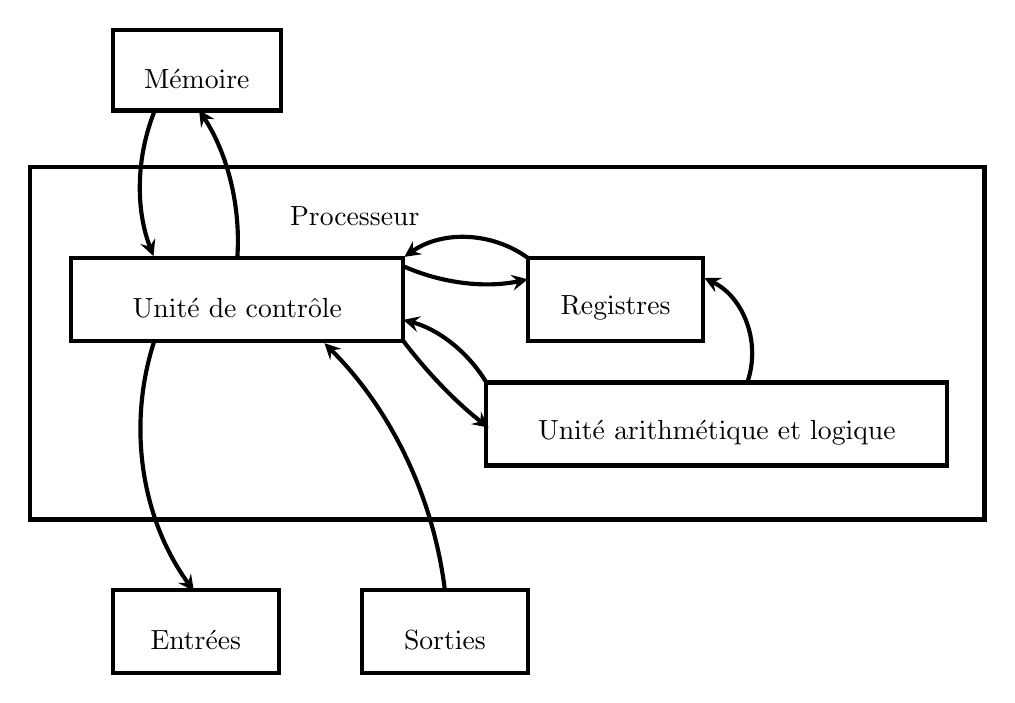
\begin{tikzpicture}
\pgftransformxscale{1.000000}
\pgftransformyscale{-1.000000}
\definecolor{dialinecolor}{rgb}{0.000000, 0.000000, 0.000000}
\pgfsetstrokecolor{dialinecolor}
\definecolor{dialinecolor}{rgb}{1.000000, 1.000000, 1.000000}
\pgfsetfillcolor{dialinecolor}
\definecolor{dialinecolor}{rgb}{1.000000, 1.000000, 1.000000}
\pgfsetfillcolor{dialinecolor}
\fill (16.000000\du,5.800000\du)--(16.000000\du,14.300000\du)--(39.000000\du,14.300000\du)--(39.000000\du,5.800000\du)--cycle;
\pgfsetlinewidth{0.100000\du}
\pgfsetdash{}{0pt}
\pgfsetdash{}{0pt}
\pgfsetmiterjoin
\definecolor{dialinecolor}{rgb}{0.000000, 0.000000, 0.000000}
\pgfsetstrokecolor{dialinecolor}
\draw (16.000000\du,5.800000\du)--(16.000000\du,14.300000\du)--(39.000000\du,14.300000\du)--(39.000000\du,5.800000\du)--cycle;
% setfont left to latex
\definecolor{dialinecolor}{rgb}{0.000000, 0.000000, 0.000000}
\pgfsetstrokecolor{dialinecolor}
\node[anchor=west] at (16.450000\du,10.245000\du){};
% setfont left to latex
\definecolor{dialinecolor}{rgb}{0.000000, 0.000000, 0.000000}
\pgfsetstrokecolor{dialinecolor}
\node[anchor=west] at (22.000000\du,7.000000\du){Processeur};
\definecolor{dialinecolor}{rgb}{1.000000, 1.000000, 1.000000}
\pgfsetfillcolor{dialinecolor}
\fill (17.000000\du,8.000000\du)--(17.000000\du,10.000000\du)--(25.000000\du,10.000000\du)--(25.000000\du,8.000000\du)--cycle;
\pgfsetlinewidth{0.100000\du}
\pgfsetdash{}{0pt}
\pgfsetdash{}{0pt}
\pgfsetmiterjoin
\definecolor{dialinecolor}{rgb}{0.000000, 0.000000, 0.000000}
\pgfsetstrokecolor{dialinecolor}
\draw (17.000000\du,8.000000\du)--(17.000000\du,10.000000\du)--(25.000000\du,10.000000\du)--(25.000000\du,8.000000\du)--cycle;
% setfont left to latex
\definecolor{dialinecolor}{rgb}{0.000000, 0.000000, 0.000000}
\pgfsetstrokecolor{dialinecolor}
\node at (21.000000\du,9.206667\du){Unité de contrôle};
\definecolor{dialinecolor}{rgb}{1.000000, 1.000000, 1.000000}
\pgfsetfillcolor{dialinecolor}
\fill (27.000000\du,11.000000\du)--(27.000000\du,13.000000\du)--(38.102500\du,13.000000\du)--(38.102500\du,11.000000\du)--cycle;
\pgfsetlinewidth{0.100000\du}
\pgfsetdash{}{0pt}
\pgfsetdash{}{0pt}
\pgfsetmiterjoin
\definecolor{dialinecolor}{rgb}{0.000000, 0.000000, 0.000000}
\pgfsetstrokecolor{dialinecolor}
\draw (27.000000\du,11.000000\du)--(27.000000\du,13.000000\du)--(38.102500\du,13.000000\du)--(38.102500\du,11.000000\du)--cycle;
% setfont left to latex
\definecolor{dialinecolor}{rgb}{0.000000, 0.000000, 0.000000}
\pgfsetstrokecolor{dialinecolor}
\node at (32.551250\du,12.206667\du){Unité arithmétique et logique};
\definecolor{dialinecolor}{rgb}{1.000000, 1.000000, 1.000000}
\pgfsetfillcolor{dialinecolor}
\fill (28.000000\du,8.000000\du)--(28.000000\du,10.000000\du)--(32.225000\du,10.000000\du)--(32.225000\du,8.000000\du)--cycle;
\pgfsetlinewidth{0.100000\du}
\pgfsetdash{}{0pt}
\pgfsetdash{}{0pt}
\pgfsetmiterjoin
\definecolor{dialinecolor}{rgb}{0.000000, 0.000000, 0.000000}
\pgfsetstrokecolor{dialinecolor}
\draw (28.000000\du,8.000000\du)--(28.000000\du,10.000000\du)--(32.225000\du,10.000000\du)--(32.225000\du,8.000000\du)--cycle;
% setfont left to latex
\definecolor{dialinecolor}{rgb}{0.000000, 0.000000, 0.000000}
\pgfsetstrokecolor{dialinecolor}
\node at (30.112500\du,9.206667\du){Registres};
\pgfsetlinewidth{0.100000\du}
\pgfsetdash{}{0pt}
\pgfsetdash{}{0pt}
\pgfsetbuttcap
{
\definecolor{dialinecolor}{rgb}{0.000000, 0.000000, 0.000000}
\pgfsetfillcolor{dialinecolor}
% was here!!!
\pgfsetarrowsend{stealth}
\definecolor{dialinecolor}{rgb}{0.000000, 0.000000, 0.000000}
\pgfsetstrokecolor{dialinecolor}
\pgfpathmoveto{\pgfpoint{28.000033\du}{8.000024\du}}
\pgfpatharc{306}{235}{2.561783\du and 2.561783\du}
\pgfusepath{stroke}
}
\pgfsetlinewidth{0.100000\du}
\pgfsetdash{}{0pt}
\pgfsetdash{}{0pt}
\pgfsetbuttcap
{
\definecolor{dialinecolor}{rgb}{0.000000, 0.000000, 0.000000}
\pgfsetfillcolor{dialinecolor}
% was here!!!
\pgfsetarrowsend{stealth}
\definecolor{dialinecolor}{rgb}{0.000000, 0.000000, 0.000000}
\pgfsetstrokecolor{dialinecolor}
\pgfpathmoveto{\pgfpoint{27.000016\du}{11.000026\du}}
\pgfpatharc{329}{285}{3.342444\du and 3.342444\du}
\pgfusepath{stroke}
}
\pgfsetlinewidth{0.100000\du}
\pgfsetdash{}{0pt}
\pgfsetdash{}{0pt}
\pgfsetbuttcap
{
\definecolor{dialinecolor}{rgb}{0.000000, 0.000000, 0.000000}
\pgfsetfillcolor{dialinecolor}
% was here!!!
\pgfsetarrowsend{stealth}
\definecolor{dialinecolor}{rgb}{0.000000, 0.000000, 0.000000}
\pgfsetstrokecolor{dialinecolor}
\pgfpathmoveto{\pgfpoint{24.999562\du}{9.999435\du}}
\pgfpatharc{143}{128}{11.225061\du and 11.225061\du}
\pgfusepath{stroke}
}
\definecolor{dialinecolor}{rgb}{1.000000, 1.000000, 1.000000}
\pgfsetfillcolor{dialinecolor}
\fill (18.000000\du,2.503333\du)--(18.000000\du,4.450000\du)--(22.045000\du,4.450000\du)--(22.045000\du,2.503333\du)--cycle;
\pgfsetlinewidth{0.100000\du}
\pgfsetdash{}{0pt}
\pgfsetdash{}{0pt}
\pgfsetmiterjoin
\definecolor{dialinecolor}{rgb}{0.000000, 0.000000, 0.000000}
\pgfsetstrokecolor{dialinecolor}
\draw (18.000000\du,2.503333\du)--(18.000000\du,4.450000\du)--(22.045000\du,4.450000\du)--(22.045000\du,2.503333\du)--cycle;
% setfont left to latex
\definecolor{dialinecolor}{rgb}{0.000000, 0.000000, 0.000000}
\pgfsetstrokecolor{dialinecolor}
\node at (20.022500\du,3.683333\du){Mémoire};
\definecolor{dialinecolor}{rgb}{1.000000, 1.000000, 1.000000}
\pgfsetfillcolor{dialinecolor}
\fill (18.000000\du,16.000000\du)--(18.000000\du,18.000000\du)--(22.000000\du,18.000000\du)--(22.000000\du,16.000000\du)--cycle;
\pgfsetlinewidth{0.100000\du}
\pgfsetdash{}{0pt}
\pgfsetdash{}{0pt}
\pgfsetmiterjoin
\definecolor{dialinecolor}{rgb}{0.000000, 0.000000, 0.000000}
\pgfsetstrokecolor{dialinecolor}
\draw (18.000000\du,16.000000\du)--(18.000000\du,18.000000\du)--(22.000000\du,18.000000\du)--(22.000000\du,16.000000\du)--cycle;
% setfont left to latex
\definecolor{dialinecolor}{rgb}{0.000000, 0.000000, 0.000000}
\pgfsetstrokecolor{dialinecolor}
\node at (20.000000\du,17.206667\du){Entrées};
\definecolor{dialinecolor}{rgb}{1.000000, 1.000000, 1.000000}
\pgfsetfillcolor{dialinecolor}
\fill (24.000000\du,16.000000\du)--(24.000000\du,18.000000\du)--(28.000000\du,18.000000\du)--(28.000000\du,16.000000\du)--cycle;
\pgfsetlinewidth{0.100000\du}
\pgfsetdash{}{0pt}
\pgfsetdash{}{0pt}
\pgfsetmiterjoin
\definecolor{dialinecolor}{rgb}{0.000000, 0.000000, 0.000000}
\pgfsetstrokecolor{dialinecolor}
\draw (24.000000\du,16.000000\du)--(24.000000\du,18.000000\du)--(28.000000\du,18.000000\du)--(28.000000\du,16.000000\du)--cycle;
% setfont left to latex
\definecolor{dialinecolor}{rgb}{0.000000, 0.000000, 0.000000}
\pgfsetstrokecolor{dialinecolor}
\node at (26.000000\du,17.206667\du){Sorties};
\pgfsetlinewidth{0.100000\du}
\pgfsetdash{}{0pt}
\pgfsetdash{}{0pt}
\pgfsetbuttcap
{
\definecolor{dialinecolor}{rgb}{0.000000, 0.000000, 0.000000}
\pgfsetfillcolor{dialinecolor}
% was here!!!
\pgfsetarrowsend{stealth}
\definecolor{dialinecolor}{rgb}{0.000000, 0.000000, 0.000000}
\pgfsetstrokecolor{dialinecolor}
\pgfpathmoveto{\pgfpoint{19.011333\du}{4.449795\du}}
\pgfpatharc{202}{159}{4.783839\du and 4.783839\du}
\pgfusepath{stroke}
}
\pgfsetlinewidth{0.100000\du}
\pgfsetdash{}{0pt}
\pgfsetdash{}{0pt}
\pgfsetbuttcap
{
\definecolor{dialinecolor}{rgb}{0.000000, 0.000000, 0.000000}
\pgfsetfillcolor{dialinecolor}
% was here!!!
\pgfsetarrowsend{stealth}
\definecolor{dialinecolor}{rgb}{0.000000, 0.000000, 0.000000}
\pgfsetstrokecolor{dialinecolor}
\pgfpathmoveto{\pgfpoint{20.999967\du}{8.000604\du}}
\pgfpatharc{4}{-33}{5.798338\du and 5.798338\du}
\pgfusepath{stroke}
}
\pgfsetlinewidth{0.100000\du}
\pgfsetdash{}{0pt}
\pgfsetdash{}{0pt}
\pgfsetbuttcap
{
\definecolor{dialinecolor}{rgb}{0.000000, 0.000000, 0.000000}
\pgfsetfillcolor{dialinecolor}
% was here!!!
\pgfsetarrowsend{stealth}
\definecolor{dialinecolor}{rgb}{0.000000, 0.000000, 0.000000}
\pgfsetstrokecolor{dialinecolor}
\pgfpathmoveto{\pgfpoint{19.000096\du}{9.999695\du}}
\pgfpatharc{198}{144}{6.720258\du and 6.720258\du}
\pgfusepath{stroke}
}
\pgfsetlinewidth{0.100000\du}
\pgfsetdash{}{0pt}
\pgfsetdash{}{0pt}
\pgfsetbuttcap
{
\definecolor{dialinecolor}{rgb}{0.000000, 0.000000, 0.000000}
\pgfsetfillcolor{dialinecolor}
% was here!!!
\pgfsetarrowsend{stealth}
\definecolor{dialinecolor}{rgb}{0.000000, 0.000000, 0.000000}
\pgfsetstrokecolor{dialinecolor}
\pgfpathmoveto{\pgfpoint{26.000003\du}{16.000021\du}}
\pgfpatharc{353}{315}{10.161156\du and 10.161156\du}
\pgfusepath{stroke}
}
\pgfsetlinewidth{0.100000\du}
\pgfsetdash{}{0pt}
\pgfsetdash{}{0pt}
\pgfsetbuttcap
{
\definecolor{dialinecolor}{rgb}{0.000000, 0.000000, 0.000000}
\pgfsetfillcolor{dialinecolor}
% was here!!!
\pgfsetarrowsend{stealth}
\definecolor{dialinecolor}{rgb}{0.000000, 0.000000, 0.000000}
\pgfsetstrokecolor{dialinecolor}
\pgfpathmoveto{\pgfpoint{24.999678\du}{8.199859\du}}
\pgfpatharc{114}{78}{4.877392\du and 4.877392\du}
\pgfusepath{stroke}
}
\pgfsetlinewidth{0.100000\du}
\pgfsetdash{}{0pt}
\pgfsetdash{}{0pt}
\pgfsetbuttcap
{
\definecolor{dialinecolor}{rgb}{0.000000, 0.000000, 0.000000}
\pgfsetfillcolor{dialinecolor}
% was here!!!
\pgfsetarrowsend{stealth}
\definecolor{dialinecolor}{rgb}{0.000000, 0.000000, 0.000000}
\pgfsetstrokecolor{dialinecolor}
\pgfpathmoveto{\pgfpoint{33.300602\du}{10.953459\du}}
\pgfpatharc{18}{-64}{2.044555\du and 2.044555\du}
\pgfusepath{stroke}
}
\end{tikzpicture}

\caption{Architecture de Harvard modifiée}
\label{fig:arch_harvard_mod}
\end{center}
\end{figure}

\paragraph{Jeu d'instructions.}
Les processeurs Intel \xq\ utilisent un jeu d'instruction complexe (CISC). La représentation d'une instruction en une suite d'octets inclut principalement un type opération (opcode\todo{opcode?}) et ses arguments. Des informations supplémentaire peuvent être codées dans l'instruction, comme des préfixes. Le format des instructions détaillé est donné figure \ref{fig:format_insts_x86}. 
L'instruction \texttt{mov ecx, 0x080490a4} de la figure \ref{fig:text_helloworld}, codée sur \texttt{b9 a4 90 04 08} est composée de l'opcode \texttt{b8+r} indiquant une opération de copie d'une valeur immédiate vers un registre. Ici le modificateur r est égal à 1, ce qui indique que le registre concerné est ecx. La valeur à copier vers le registre est 0x080490a4 soient les octets \texttt{a4 90 04 08} codés en petit-boutistes \todo{endianness ??}, c'est à dire que les mots de poids faibles sont écrits en premiers, à l'inverse de l'écriture usuelle.
Il s'agit d'une assignation immédiate et la valeur à copier vers \texttt{ecx} est la valeur immédiate.
Le décalage permet de modifier une instruction d'adressage indirect comme \texttt{mov ecx, [eax]}, écrivant le contenu en mémoire à l'adresse \texttt{eax} dans le registre \texttt{ecx} en \texttt{mov ebx, [eax+d]} où \texttt{d} est le décalage.
Enfin les préfixes permettent par exemple de répéter plusieurs fois l'instruction jusqu'à ce qu'une condition sur un registre soit remplie.

\begin{figure}
\begin{center} 
\begin{tabular}{|c|c|c|c|c|c|}
\hline
% Prefixe & Opcode & Modificateur & SIB & Déplacement d'octet & Adressage\\
% 1 à 4 & 1 à 3 & 0 ou 1 & 0 ou 1 & 0 à 4 & 0 à 4\\
Prefixe & Opcode & Modificateur & Décalage & Valeur immédiate\\
1 à 4 & 1 à 3 & 0 à 2 & 0 à 4 & 0 à 4\\
\hline
\end{tabular}
\end{center} 
\caption{Format d'une instruction \xq}
\label{fig:format_insts_x86}
\end{figure}

\section{Obfuscations}
\subsection{Auto-modification}
\todo[inline]{
Qu'est-ce ? \\
Autorisé par l'OS (NX ?) \\
Comment ? \\
Exemple
}

\subsection{Obscurcissement statique}
\todo[inline]{
Ajout de junk code \\
Réorganisation du code \\
Aplatissement de CFG \\
Détournement de calls \\
Chevauchements \\
}
